\documentclass[tikz,border=12pt]{standalone}
\usepackage[T1]{fontenc}
\usepackage{tgheros}
\usepackage{sfmath}
\usepackage{amsmath,amssymb}
% % \usepackage{fontawesome5} (Removed for publication-grade academic typography) (Removed for publication-grade academic typography)
\usepackage{tikz}
\usetikzlibrary{arrows.meta,positioning,shapes.geometric,fit,backgrounds,calc,decorations.pathreplacing}
\usepackage{xcolor}

\renewcommand{\familydefault}{\sfdefault}

% Academic Semantic Palette
\definecolor{ethdarkblue}{HTML}{1B2A4A}
\definecolor{ethslate}{HTML}{475569}
\definecolor{cardbg}{HTML}{F8FAFC}
\definecolor{cardborder}{HTML}{CBD5E1}
\definecolor{measuredTeal}{HTML}{168F84}
\definecolor{tealBg}{HTML}{E4F6F3}
\definecolor{proposalAmber}{HTML}{C98218}
\definecolor{amberBg}{HTML}{FFF3DC}
\definecolor{consequenceCoral}{HTML}{BD4F2F}
\definecolor{coralBg}{HTML}{FAE9E2}
\definecolor{authorityViolet}{HTML}{6550A8}
\definecolor{violetBg}{HTML}{F0ECFA}

\begin{document}
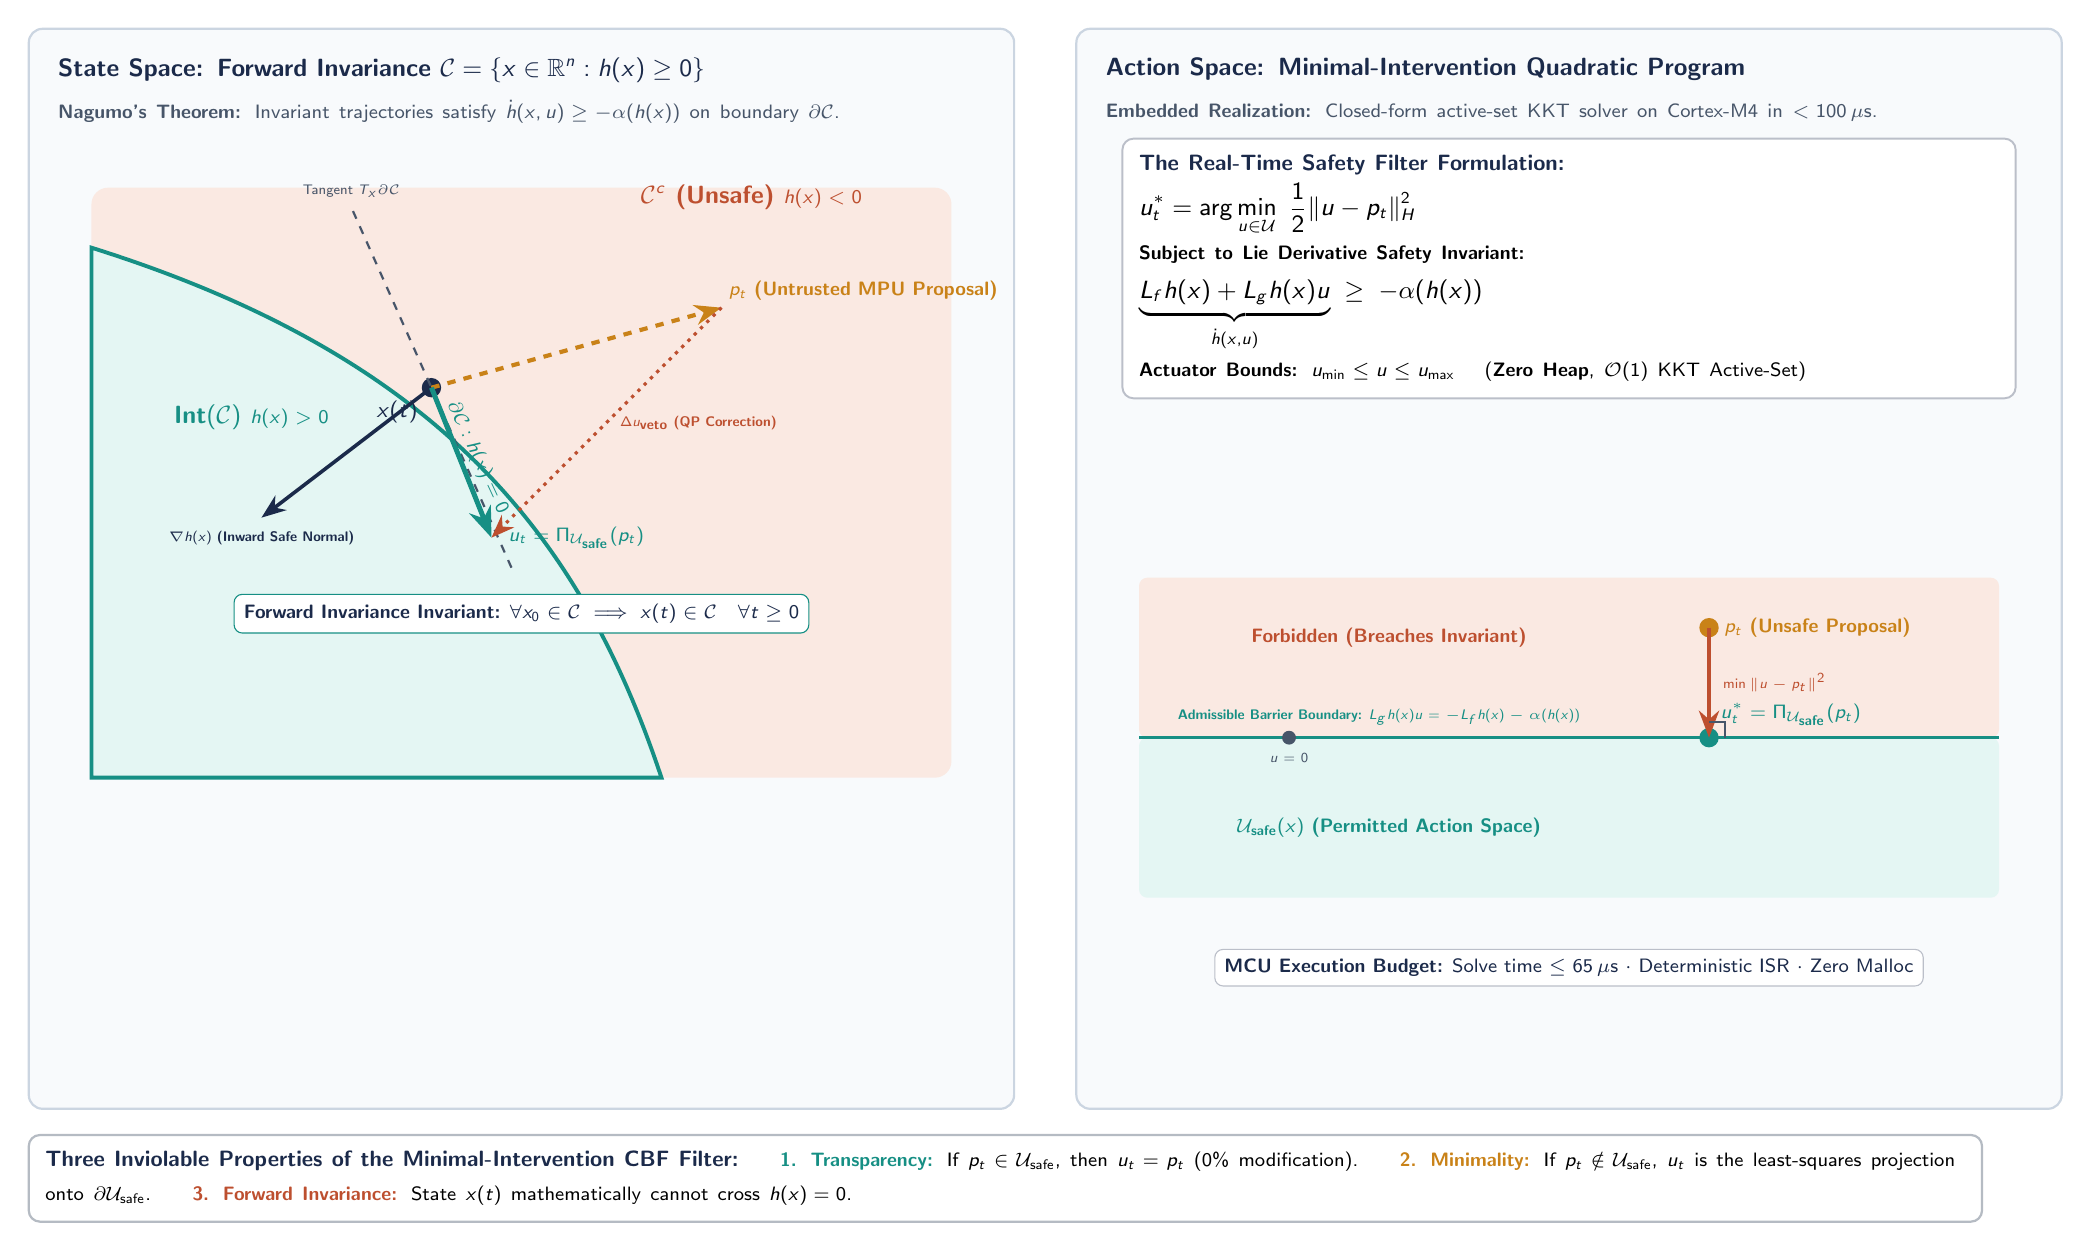
\begin{tikzpicture}[
  font=\sffamily,
  >=Stealth
]

  % --- LEFT CARD CONTAINER ---
  \node[draw=cardborder, fill=cardbg, rounded corners=5pt, line width=0.8pt, text width=4.65in, minimum height=5.40in, inner sep=10pt, anchor=north west] (card_left) at (0, 0) {};
  
  % Header for Left Card
  \node[anchor=north west, text width=4.40in, align=left, inner sep=0pt] at ($(card_left.north west)+(0.15in, -0.15in)$) {
    {\small\bfseries\color{ethdarkblue} State Space: Forward Invariance $\mathcal{C} = \{x \in \mathbb{R}^n : h(x) \ge 0\}$}\\[3pt]
    {\scriptsize\color{ethslate}\textbf{Nagumo's Theorem:} Invariant trajectories satisfy $\dot{h}(x, u) \ge -\alpha(h(x))$ on boundary $\partial\mathcal{C}$.}
  };

  % Center coordinate for Left Drawing
  \coordinate (Lcenter) at ($(card_left.north)+(0, -2.15in)$);

  % Unsafe Region Background
  \fill[coralBg, rounded corners=6pt] ($(Lcenter)+(-2.15in,-1.60in)$) rectangle ($(Lcenter)+(2.15in,1.35in)$);

  % Safe Set Region (Curved super-level set)
  \fill[tealBg, draw=measuredTeal, line width=1.4pt] 
    ($(Lcenter)+(-2.15in,-1.60in)$) -- 
    ($(Lcenter)+(0.70in,-1.60in)$) .. controls ($(Lcenter)+(0.30in,-0.40in)$) and ($(Lcenter)+(-0.40in,0.50in)$) .. 
    ($(Lcenter)+(-2.15in,1.05in)$) -- cycle;

  % Boundary Label (h(x) = 0)
  \node[font=\sffamily\bfseries\scriptsize, text=measuredTeal, rotate=-65] at ($(Lcenter)+(-0.22in, 0.00in)$) {
    $\partial \mathcal{C}: h(x) = 0$
  };

  % Safe Interior Label
  \node[font=\sffamily\bfseries\small, text=measuredTeal] at ($(Lcenter)+(-1.35in, 0.20in)$) {
     $\text{Int}(\mathcal{C})$\\[1pt]
    {\scriptsize $h(x) > 0$}
  };

  % Unsafe Region Label
  \node[font=\sffamily\bfseries\small, text=consequenceCoral] at ($(Lcenter)+(1.15in, 1.30in)$) {
     $\mathcal{C}^c$ (Unsafe)\\[1pt]
    {\scriptsize $h(x) < 0$}
  };

  % Current State Point x(t)
  \coordinate (x0) at ($(Lcenter)+(-0.45in, 0.35in)$);
  \fill[ethdarkblue] (x0) circle (3.5pt) node[below left=2pt, font=\sffamily\bfseries\footnotesize, text=ethdarkblue] {$x(t)$};

  % Inward Normal nabla h(x)
  \draw[->, line width=1.3pt, ethdarkblue] (x0) -- ++(-0.85in, -0.65in)
    node[below=1pt, font=\sffamily\bfseries\tiny, text=ethdarkblue] {$\nabla h(x)$ (Inward Safe Normal)};

  % Tangent Hyperplane at x(t)
  \draw[dashed, line width=0.8pt, ethslate] ($(x0)+(0.40in,-0.90in)$) -- ($(x0)+(-0.40in,0.90in)$)
    node[above, font=\sffamily\tiny, text=ethslate] {Tangent $T_x \partial\mathcal{C}$};

  % Neural Proposal Vector p_t (Pointing toward unsafe region)
  \draw[->, dashed, line width=1.5pt, proposalAmber] (x0) -- ++(1.45in, 0.40in)
    node[above right=-2pt, font=\sffamily\bfseries\scriptsize, text=proposalAmber] {$p_t$ (Untrusted MPU Proposal)};

  % Minimal Projected Command u_t (Along tangent boundary into safe half-space)
  \draw[->, line width=1.8pt, measuredTeal] (x0) -- ++(0.30in, -0.75in)
    node[right=2pt, font=\sffamily\bfseries\scriptsize, text=measuredTeal] {$u_t = \Pi_{\mathcal{U}_{\text{safe}}}(p_t)$};

  % Vetoed Delta Vector (Correction)
  \draw[->, dotted, line width=1.2pt, consequenceCoral] ($(x0)+(1.45in, 0.40in)$) -- ($(x0)+(0.30in, -0.75in)$)
    node[midway, right=1pt, font=\sffamily\bfseries\tiny, text=consequenceCoral] {$\Delta u_{\text{veto}}$ (QP Correction)};

  % State Invariant Formula Badge at bottom of left card
  \node[draw=measuredTeal, fill=white, rounded corners=3pt, font=\sffamily\scriptsize, text=ethdarkblue, inner sep=3.5pt] at ($(Lcenter)+(0, -0.78in)$) {
    \textbf{Forward Invariance Invariant:} $\forall x_0 \in \mathcal{C} \implies x(t) \in \mathcal{C} \quad \forall t \ge 0$
  };


  % --- RIGHT CARD CONTAINER ---
  \node[draw=cardborder, fill=cardbg, rounded corners=5pt, line width=0.8pt, text width=4.65in, minimum height=5.40in, inner sep=10pt, right=0.30in of card_left.north east, anchor=north west] (card_right) {};

  % Header for Right Card
  \node[anchor=north west, text width=4.40in, align=left, inner sep=0pt] at ($(card_right.north west)+(0.15in, -0.15in)$) {
    {\small\bfseries\color{ethdarkblue} Action Space: Minimal-Intervention Quadratic Program}\\[3pt]
    {\scriptsize\color{ethslate}\textbf{Embedded Realization:} Closed-form active-set KKT solver on Cortex-M4 in $<100\,\mu\text{s}$.}
  };

  % QP Optimization Formulation Box
  \node[draw=ethdarkblue!30, fill=white, rounded corners=4pt, line width=0.7pt, text width=4.30in, inner sep=6pt, align=left, below=0.55in of card_right.north] (qp_box) {
    {\footnotesize\bfseries\color{ethdarkblue}The Real-Time Safety Filter Formulation:}\\[2pt]
    {\small $\displaystyle u_t^* = \arg\min_{u \in \mathcal{U}} \; \frac{1}{2} \| u - p_t \|_H^2$}\\[4pt]
    {\scriptsize\textbf{Subject to Lie Derivative Safety Invariant:}}\\[2pt]
    {\small $\displaystyle \underbrace{L_f h(x) + L_g h(x) u}_{\dot{h}(x, u)} \;\ge\; -\alpha(h(x))$}\\[3pt]
    {\scriptsize\textbf{Actuator Bounds:} $u_{\min} \le u \le u_{\max}$ \quad (\textbf{Zero Heap}, $\mathcal{O}(1)$ KKT Active-Set)}
  };

  % Center coordinate for Right Drawing
  \coordinate (Rcenter) at ($(card_right.north)+(0, -3.55in)$);

  % Forbidden Half-Plane (Top)
  \fill[coralBg, rounded corners=3pt] ($(Rcenter)+(-2.15in,0)$) rectangle ($(Rcenter)+(2.15in,0.80in)$);
  % Admissible Half-Plane (Bottom)
  \fill[tealBg, rounded corners=3pt] ($(Rcenter)+(-2.15in,-0.80in)$) rectangle ($(Rcenter)+(2.15in,0)$);

  % Barrier Hyperplane in Action Space: a_cbf^T u = b_cbf
  \draw[line width=1.3pt, measuredTeal] ($(Rcenter)+(-2.15in,0)$) -- ($(Rcenter)+(2.15in,0)$)
    node[pos=0.03, above right=1pt, font=\sffamily\bfseries\tiny, text=measuredTeal] {Admissible Barrier Boundary: $L_g h(x) u = -L_f h(x) - \alpha(h(x))$};

  % Origin in Action Space
  \coordinate (u_orig) at ($(Rcenter)+(-1.40in, 0)$);
  \fill[ethslate] (u_orig) circle (2.5pt) node[below=2pt, font=\sffamily\tiny, text=ethslate] {$u = 0$};

  % Candidate Proposal p_t (In Forbidden Half-Plane)
  \coordinate (u_prop) at ($(Rcenter)+(0.70in, 0.55in)$);
  \fill[proposalAmber] (u_prop) circle (3.5pt)
    node[right=2pt, font=\sffamily\bfseries\scriptsize, text=proposalAmber] {$p_t$ (Unsafe Proposal)};

  % Projected Permitted Control u_t* (Orthogonal Projection on Hyperplane)
  \coordinate (u_proj) at ($(Rcenter)+(0.70in, 0)$);
  \fill[measuredTeal] (u_proj) circle (3.5pt)
    node[above right=1pt, font=\sffamily\bfseries\scriptsize, text=measuredTeal] {$u_t^* = \Pi_{\mathcal{U}_{\text{safe}}}(p_t)$};

  % Orthogonal Projection Vector
  \draw[->, line width=1.5pt, consequenceCoral] (u_prop) -- (u_proj)
    node[midway, right=1pt, font=\sffamily\bfseries\tiny, text=consequenceCoral] {$\min \|u - p_t\|^2$};

  % Right Angle Symbol
  \draw[line width=0.6pt, ethslate] ($(u_proj)+(0.08in,0)$) -- ($(u_proj)+(0.08in,0.08in)$) -- ($(u_proj)+(0,0.08in)$);

  % Region Text
  \node[font=\sffamily\bfseries\scriptsize, text=consequenceCoral] at ($(Rcenter)+(-0.90in, 0.50in)$) {
    Forbidden (Breaches Invariant)
  };
  \node[font=\sffamily\bfseries\scriptsize, text=measuredTeal] at ($(Rcenter)+(-0.90in, -0.45in)$) {
    $\mathcal{U}_{\text{safe}}(x)$ (Permitted Action Space)
  };

  % Performance Summary Badge
  \node[draw=ethdarkblue!30, fill=white, rounded corners=3pt, font=\sffamily\scriptsize, text=ethdarkblue, inner sep=3.5pt] at ($(Rcenter)+(0, -1.15in)$) {
    \textbf{MCU Execution Budget:} Solve time $\le 65\,\mu\text{s}$ $\cdot$ Deterministic ISR $\cdot$ Zero Malloc
  };

  % --- BOTTOM STRIP ---
  \node[draw=ethslate!40, fill=white, rounded corners=4pt, line width=0.8pt, text width=9.60in, inner sep=6pt, below=0.12in of card_left.south west, anchor=north west] (strip) {
    {\footnotesize\textbf{\color{ethdarkblue}Three Inviolable Properties of the Minimal-Intervention CBF Filter:}} \quad
    {\scriptsize\textbf{\color{measuredTeal}1. Transparency:}} {\scriptsize If $p_t \in \mathcal{U}_{\text{safe}}$, then $u_t = p_t$ ($0\%$ modification).} \quad
    {\scriptsize\textbf{\color{proposalAmber}2. Minimality:}} {\scriptsize If $p_t \notin \mathcal{U}_{\text{safe}}$, $u_t$ is the least-squares projection onto $\partial\mathcal{U}_{\text{safe}}$.} \quad
    {\scriptsize\textbf{\color{consequenceCoral}3. Forward Invariance:}} {\scriptsize State $x(t)$ mathematically cannot cross $h(x)=0$.}
  };

\end{tikzpicture}
\end{document}
